%%%%%%%%%%% Aquí va la solución al problema 2.
\newpage
\textbf{\textcolor{MidnightBlue}{2.}}
Considera un sistema distribuido representado como una gráfica de tipo anillo, cuyos
canales son bidireccionales, con n = mk procesos, con $m > 1$ y $k$ es impar. Los procesos en las
posiciones $0,\; k,\; 2k, . . . ,(m-1)k$ son marcados inicialmente como líderes, mientras que procesos
en otras posiciones son seguidores. Todos los procesos tienen un sentido de dirección y pueden
distinguir su vecino izquierdo de su vecino derecho, pero ellos no tienen información alguna
acerca de sus ids. \newline

El algoritmo $1$ está destinado a permitir que los líderes recluten seguidores. No es difícil ver que
todo seguidor eventualmente se agrega a sí mismo a un árbol enraízado con padre en algún líder.
Nos gustaría que todos esos árboles tuvieran aproximadamente el mismo número de nodos.

\begin{itemize}
\item ¿Cuál es el tamaño mínimo y máximo posible de un árbol?
      
\item Dibuja el resultado de una ejecución para el algoritmo con $k = 5$  y $m = 4.$
      
\end{itemize}

\begin{figure}[ht]
        \begin{center}
                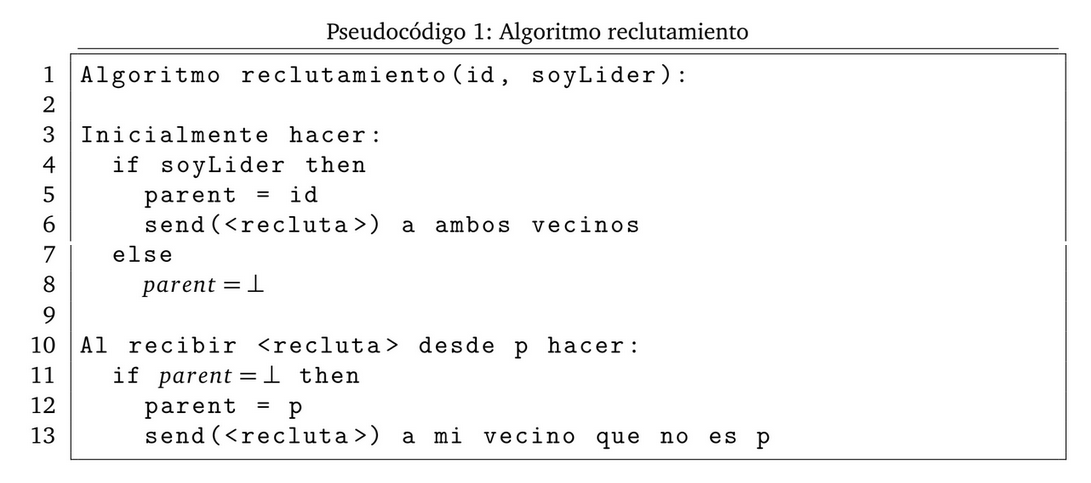
\includegraphics[width=15cm]{AlgReclutamiento.png}
        \end{center}
\end{figure}

%%%%%%%% Solución:
$\rhd$ Empecemos dando respuesta a la pregunta ¿Cuál es el tamaño mínimo y máximo posible de un árbol?.
Para contestar esta pregunta análicemos varias cosas:
\begin{enumerate}
\item Sabemos que la cantidad de procesos es múltiplo de la cantidad de líderes, pues si
      
      \[n, m, k \in \mathbb{N} \Rightarrow \frac{n}{k} = m \in \mathbb{N}.\]
      
      Entonces, la cantidad de líderes ($k$) es proporcional a la cantidad de seguidores ($m$),
      hasta el momento no sabemos si a cada líder le corresponda la misma cantidad de seguidores
      basados en el algoritmo de \code{reclutamiento}.
      
\item Recordemos que $k$ es impar y por tanto tiene la forma $k = 2r + 1$ ($r \in \mathbb{N} \cup \{0\}$).
      Ahora, nos podemos preguntar ¿cada cuántos procesos hay un líder contando desde el último anterior
      o próximo? la respuesta es cada $k$ procesos y la diferencia entre estos es de $k - 1$ procesos,
      pues los líderes están ubicados en múltiplos de $k$, luego
      \[ k - 1 = (2r + 1) - 1 = 2r.\]
      Inicialmente, los procesos líderes empiezan a reclutar (línea 6). Después de la primer ronda
      los procesos reclutados reclutan a sus vecinos que no son su padre (línea 13). Eventualmente
      todo los procesos seguidores son relcutados, como todo esto (en cada proceso reclutado lo que sigue
      es reclutar a su vecino) pasa al mismo tiempo (en cada ronda los procesos líderes tienen la misma
      cantidad de descendientes) podemos notar que la diferencia de procesos entre cualesquiera dos
      procesos líderes es dividida entre $2$ para que cada líder termine por ser ancestro común de
      exactamente la mitad, adyacente al líder en cuestión, de esos procesos.

      Hasta este momento sabemos que un líder llegará a tener $r$ descendientes por lado, en total
      cada líder tendrá $2r$ descendientes.
      
\item Como los árboles están enraizados por líderes y cada líder tiene $2r$ descendientes. Entonces, el
total de nodos en los arboles generados será $2r + 1 = k$. Concluimos que el tamaño por árbol es de $k$
sin importar como es $m$ o $k$.
\end{enumerate}

Por último, veamos como se ve la gráfica después de haber ejecutado el algoritmo de \code{reclutamiento}:
\begin{figure}[ht]
        \begin{center}
                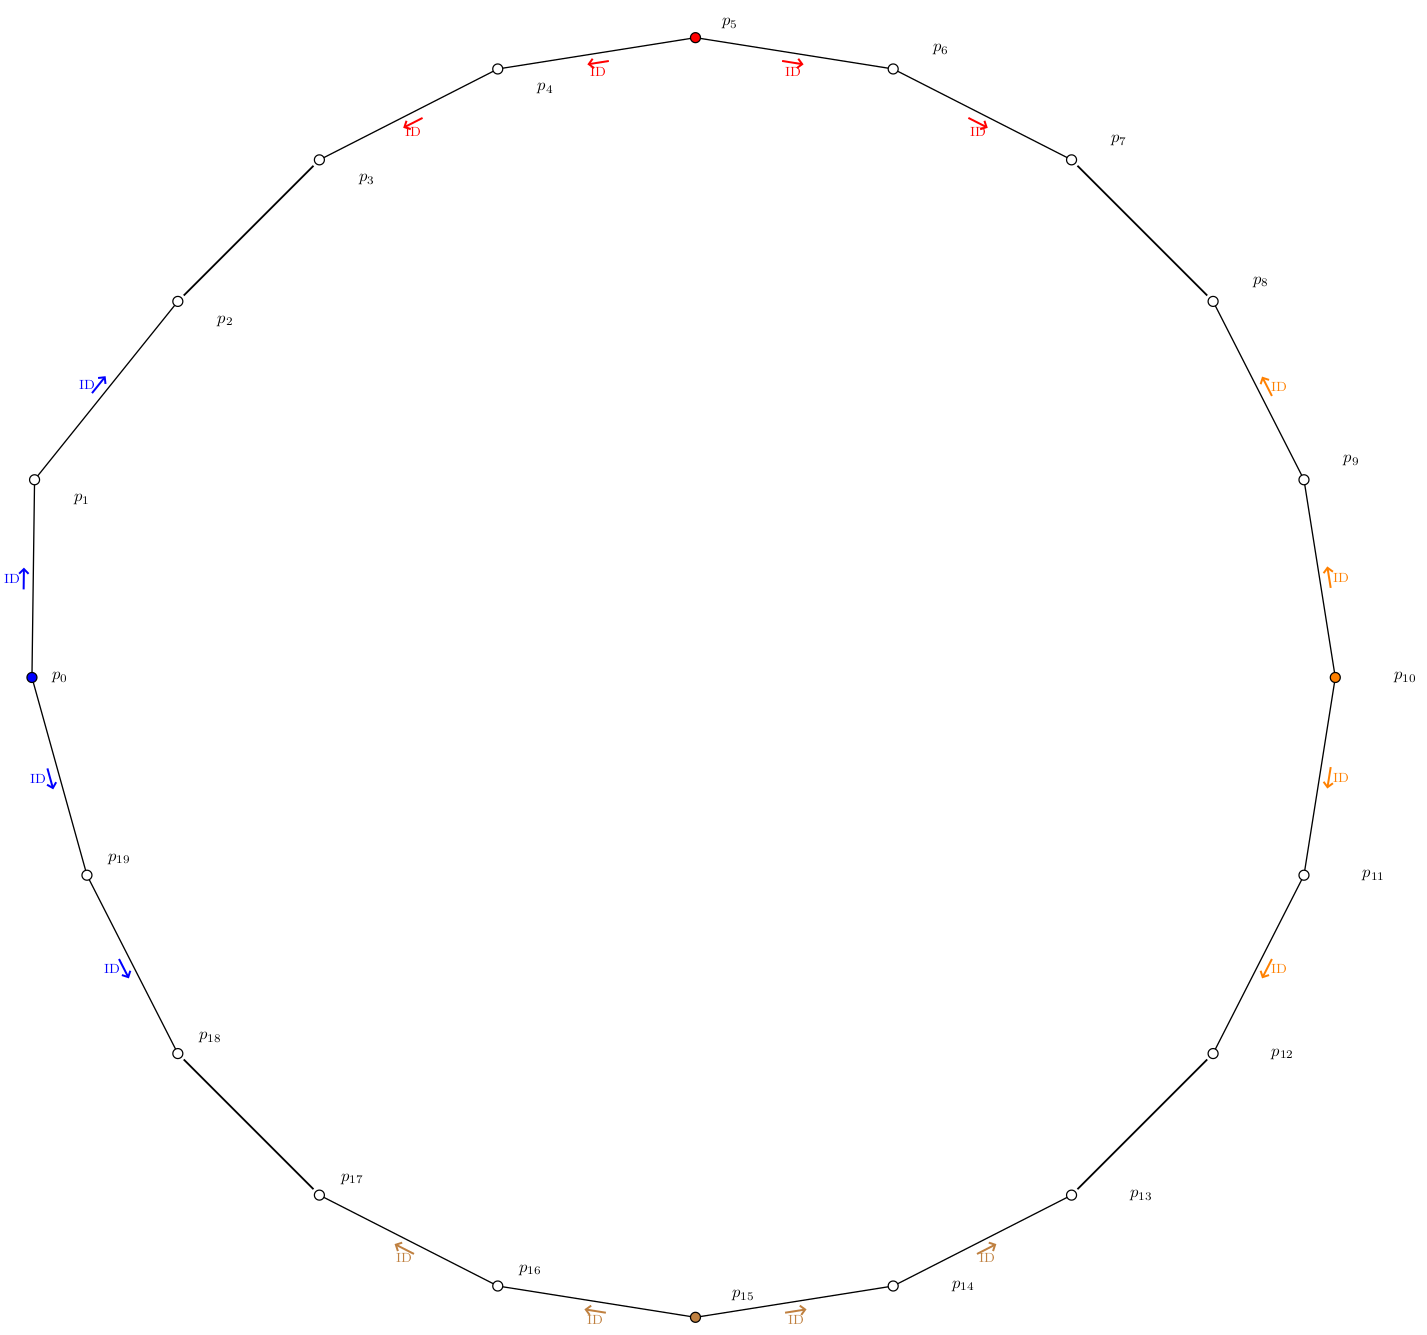
\includegraphics[width=15cm]{Ejecucion.png}
        \end{center}
\end{figure}

Los árboles en este caso se pueden formar desde cada nodo representado por algún
color\footnote{estos son los nodos distinguidos como líderes.} y hasta donde se
indica con las flechas del respectivo color.
\hfill $\lhd$
